\documentclass{article}
\usepackage{tikz}
\usepackage[margin=2cm]{geometry}
\usetikzlibrary{arrows.meta}

\begin{document}

\begin{center}
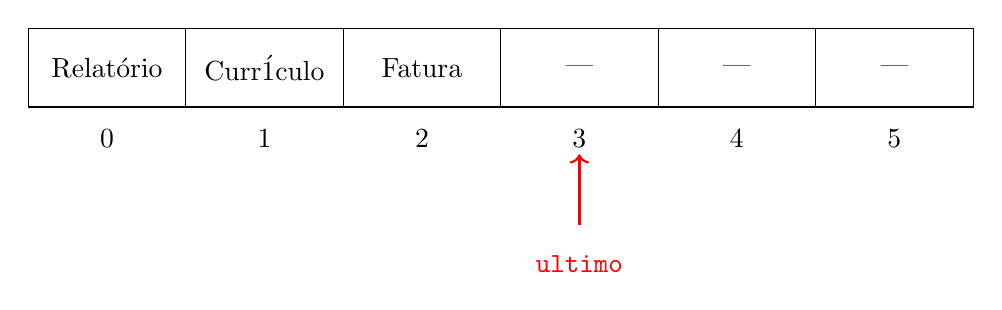
\begin{tikzpicture}[scale=1, every node/.style={scale=1}]

% Tabela com 6 elementos (0 a 5)
\foreach \i in {0,1,2,3,4,5} {
  \draw (2*\i,0) rectangle (2*\i+2,1);
  \node at (2*\i+1,0.5) {%
    \ifnum\i=0 Relatório%
    \else\ifnum\i=1 Currículo%
    \else\ifnum\i=2 Fatura%
    \else ---%
    \fi\fi\fi
  };
  \node at (2*\i+1,-0.4) {\i};
}

% Índice "ultimo"
\draw[<-, thick, red] (7,-0.6) -- (7, -1.5);
\node[red] at (7, -2) {\texttt{ultimo}};

\end{tikzpicture}
\end{center}

\end{document}
